\section{HHL Algorithmus}

%\subsubsection{Übersicht}

    \begin{frame}
    \frametitle{Übersicht}
    Vergleich klassische zur quanten Version

    \hfil

    \begin{columns}[c]
        \begin{column}{0.6\hsize}\centering
        Klassisch
        $$A \vec{x} = \vec{b}$$
        $$\vec{x} = A^{-1}\vec{b}$$
        \end{column}

        \begin{column}{0.4\hsize}
        Quanten Version
        $$A \ket{x} = \ket{b}$$
        $$\ket{x} = A^{-1}\ket{b}$$
        \end{column}
    \end{columns}

    \hfil

    \hfil
    
    Spektralzerlegung von $A$ und $\ket{b}$
    $$\ket{x} =  A^{-1} \ket{b} = \sum_{i=0}^{2^{n_b}-1} \lambda_i^{-1} b_j\ket{u_j}$$

    \end{frame}


%\subsubsection{Der Algorithmus}

    \begin{frame}
    \frametitle{Der Algorithmus}

        \textbf{Ablauf}
        \begin{enumerate}
            \item State Preparation
            \begin{itemize}
                \item Enkodiert Vektor und Matrix in Quanten Computer
            \end{itemize}
            \item Quantum Phase Estimation
            \begin{itemize}
                \item ermittelt Eigenwerte 
            \end{itemize}
            \item Ancilla Bit Rotation 
            \begin{itemize}
                \item  Invertiert Eigenwerte
            \end{itemize}
            \item Inverse Quantum Phase Estimation
             \begin{itemize}
                \item löst verschränkte Qubits auf
            \end{itemize}
            
            \item Messung
             \begin{itemize}
                \item liest das Ergebnis $\ket{x}$ aus
            \end{itemize}
 
        \end{enumerate}

    \end{frame}

\begin{frame}
    \frametitle{Quantum Circuit}
    \begin{center}
    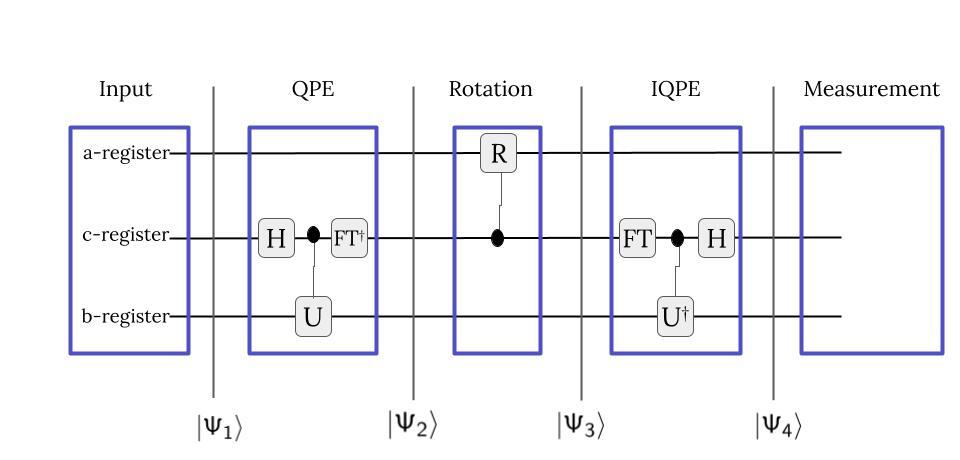
\includegraphics[width=10.5cm]{img/hhl_circuit/hhl_circuit.jpg}
    \end{center}
    \begin{enumerate}
        \item Ancilla (Helfer): a-register
        \begin{itemize}
            \item Indikator qubit, zeigt ob Zustände verschränkt sind
        \end{itemize}

        \item Register: c-register
        \begin{itemize}
            \item beinhaltet die Eigenwerte
        \end{itemize}
        
        \item Input: b-register 
        \begin{itemize}
            \item beinhaltet den Vektor $\vec{b}$
        \end{itemize}
        
    \end{enumerate}
   \end{frame}
